% !TEX root = ../Dissertation.tex
%===================================================================================================

\chapter{Discussion}

\section{Intrathymic B cell development}
The aims of this project was to further investigate the potential intrathymic development of thymic B cells seen in the NOD mouse.
The increase in B cells seen in the thymus of these mice compared to the thymus of control, nondiabetic B6 mice has prompted investigation into the mechanism by which B cells arise in the thymus.
The main hypotheses so far are development, where thymic B cells are developing from progenitors in the thymus, and migration, where B cells are being released from the bone marrow and migrating to the thymus.
However, there is overlap between these two hypotheses as, in order to develop from progenitors in the thymus, the progenitors must first migrate from the bone marrow to the thymus as the thymus has no self-renewing cells.
Therefore, it is more a question of at what point B cells are developing from in the thymus.
For example, are they developing from progenitors and committing to the B cell lineage in the thymus, are they developing from B cell committed pro or pre B cells onwards, or are they mature circulating B cells that have taken up residence in the thymus.

The general consensus is that B cells are developing within the thymus with very little contribution from the circulation.
Experiments involving parabiotic congenic mice showed that of the thymic B cells, the majority were of the endogenous phenotype, not the parabiotic partner. 
This gave the impression that the thymic B cells have more to do with the thymus itself, rather than the circulation \citep{Perera2013}.
Similarly, \citet{Akashi2000} found that when donor B cells of a different Ly5 isoform were injected into recipient mice, very few of the thymic emigrant B cells were of donor origin, suggesting that they could be more attributable to development within the host rather than a result of circulating B cells stopping in the thymus.

To investigate intrathymic B cell development, B cells were looked at at different developmental stages, such as pro and pre B cells in the thymus.
These stages are following lineage commitment.
However, the stages before were also investigated by looking for early B cell progenitors, thought to be Sca-1\textsuperscript{low}c-kit\textsuperscript{low}Flt3\textsuperscript{+}IL-7R$\alpha$\textsuperscript{+}Ly6D\textsuperscript{+} BLPs.

Pro and pre B cells are seen in the thymus.
However, it is not known whether these are developing or have migrated following premature release from the bone marrow.
To tackle this question, RAG expression was looked for in CD19\textsuperscript{+} cells in the thymus of NOD mice.
It was seen that there are populations of CD19\textsuperscript{+}RAG\textsuperscript{high}, CD19\textsuperscript{+}RAG\textsuperscript{low} and CD19\textsuperscript{+}RAG\textsuperscript{-} cells in the NOD thymus.
The RAG\textsuperscript{high} cells are very likely developing there within the thymus as this very bright signal was equivalent to that seen in actively developing T cells in the thymus.
This gives the impression that RAG is being actively transcribed in CD19\textsuperscript{+} cells in the thymus, indicating active BcR rearrangement and B cell development.

These RAG expressing CD19\textsuperscript{+} cells were looked for in NOD-RAG-GFP mice of 4, 7 and 11 weeks of age and interestingly, the CD19\textsuperscript{+}RAG\textsuperscript{high} population frequency didn't change, whereas the CD19\textsuperscript{+}RAG\textsuperscript{low} frequency decreased significantly.
This gives the impression that as mice age, there are less newly developed B cells in the thymus, potentially as a result of decreased development.
However, if development does decrease, the same is not seen in the population of B cells in the thymus, therefore, it may be that following initial development, the B cell numbers in the NOD thymus are increased due to proliferation of B cells.

To investigate this further, it would be interesting to look at the same thing in B6 mice which have a normal, small population of thymic B cells and compare both frequencies and absolute numbers between strains.
If the same pattern was seen in the B6 and the NOD, both in terms of frequency and numbers, it could suggest that the increase in B cells occurs following the development stage, for example, proliferation.

As an alternative, it may be that the decrease in CD19\textsuperscript{+}RAG\textsuperscript{low} cells is due to these newly developed B cells leaving the thymus and travelling elsewhere.
In this case, it may be that the thymus is acting like the bone marrow, harbouring B cell development then releasing immature B cells to continue development elsewhere.
The decrease also coincides with disease progression, therefore it may be that thymic B cells can contribute to the process of insulitis and move to the islets.
However, this is just speculation.
It would be beneficial to track thymic cells in order to see whether they stay within the thymus or move elsewhere.

It was also of interest that the presence of pro B cells in the NOD thymus was linked to the presence of a mature B cell.
The frequency of pro B cells was found to be significantly lower in NOD KO thymi compared to NOD WT and B6 controls.
This is of interest as it begs the question as to what the role of a mature B cell might be.
Some potential roles are outlined below:
\begin{itemize}
\item A mature B cell may be helping with the recruitment of B cell progenitors from the bone marrow to the thymus
\item A mature B cell may provide a survival factor for B cell progenitors within the thymus so that they survive to be able to development
\item A mature B cell may kick start the process of B cell transcription factor expression within the thymus, so that the thymus can provide an environment conducive to B cell development
\item A mature B cell may provide a survival factor for newly developed B cells so that once they have developed they are able to survive.
\end{itemize}

With the results of the NOD KO mouse, it is unlikely that the action of a mature B cell is following the developmental process and providing a survival factor for newly developed B cells.
If this was the case, the population of pro B cells in the thymus of KO mice would be normal.
It is more likely that it's role is earlier in the process, either B cell progenitor recruitment, kickstarting transcription factor expression or a pro B cell survival factor.

It would be interesting to investigate the influence of a mature B cell on pro B cells in NOD KO mice further.
To do this, it may be necessary to irradiate NOD KO mice then replace with NOD KO bone marrow supplemented with NOD B cells to try and avoid the B cells being killed off by CTLs that have not been tolerised to B cells during development \citep{Serreze1998}.
By adding purified mature B cells, it would be interesting to see if this was sufficient to increase pro B cell frequency in the KO thymus.
Following this, it would also be of interest to try transplanting KO bone marrow supplemented with B6 B cells to see if it is a characteristic of a NOD B cell that can increase thymic pro B cells.
It is not known whether the mature B cell needs to be of splenic or thymic origin, therefore these experiments could also test that by separately transferring bone marrow supplemented with B cells from both tissues.

CD43 expression was also found to be of interest in the NOD mouse compared to the B6 control.
It appeared that the expression of CD43 was much higher on mice of NOD background compared to B6.
The reason for this is not known, however, it is possible that CD43 provides an important tool for allowing T cells to move from the blood into lymphoid tissues.
Evidence for this was shown in 1999 by \citet{Mikulowska1999} when an anti-CD43 antibody (L11) was used following transfer of NOD splenocytes into NOD/scid recipient mice. 
Normally, this would cause T1D in the recipient mice and this was indeed seen in the control mice which did not receive L11.
However, in mice receiving L11, it was shown that the onset of T1D was significantly delayed.
It was further shown by \citet{Johnson1999} showed that L11 was capable of providing significant protection from T1D onset in NOD mice.

Considering the results showing increased CD43 expression in NOD thymi compared to B6 thymi along with these previous findings regarding anti-CD43 antibodies, it is worth considering whether T1D in the NOD mouse may be related to the levels of CD43 expressed in the NOD thymus.
It may be that the increased CD43 expression in NOD mice may be allowing the infiltration into the pancreas, something which is not seen in B6 mice.
It is worth further investigation to see if this is replicable when the group size is increased.


Following the findings that pro and pre B cells are probably developing within the thymus, shown by CD19\textsuperscript{+}RAG\textsuperscript{+} cell presence, earlier progenitors were investigated.
These Sca-1\textsuperscript{low}c-kit\textsuperscript{low}Flt3\textsuperscript{+}IL-7R$\alpha$\textsuperscript{+}Ly6D\textsuperscript{+} BLPs are believed to be the point of B cell commitment, therefore if they are present in the NOD mouse, it is possible that all stages of B cell development are occurring in the thymus.

It was wondered whether B cell progenitors, such as BLPs, would be increased in the NOD mouse compared to the B6.
When looking for potential TSPs, cells with the correct markers to allow homing were considered \citep{Zlotoff2011}, therefore, it may be that if marker expression in the bone marrow is abherrent on B cell progenitors, it may result in an excess of B cell precursors being able to migrate to the thymus alongside T cell progenitors.

It was interesting when investigating the presence of BLPs that the frequency of BLPs in the Sca-1\textsuperscript{low}c-kit\textsuperscript{low}Flt3\textsuperscript{+}IL-7R$\alpha$\textsuperscript{+} population of the thymus of the NOD mouse, was significantly decreased compared to the B6.

However, before any assumptions can be made on this data, it is first necessary to ask some questions about BLPs.
\begin{itemize}
\item Are BLPs the sole progenitor for B cell development?
\item Is B cell development from BLPs restricted only to the bone marrow?
\item Can the B cell developmental pathway from HSCs through to pro B cell in the bone marrow be applied to B cell development in the thymus?
\end{itemize}

In order to help determine the answers to the questions above, it would necessary to carry out further experiments.
To determine whether B cells can develop from BLPs in the thymus, it would be interesting to culture BLPs on thymic stromal cell lines.
This in vitro approach may be able to indicate whether or not B cells could develop from BLPs in the thymus.
However, it is unlikely that B cell development from BLPs is restricted only to the bone marrow, shown by the presence of BLPs in the B6 thymus.
These may be the way in which a normal, small population of B cells arises in the B6 thymus.

However, the NOD thymus has a significantly smaller frequency of BLPs in the thymus compared to the B6.
Despite this, NODs still have increased thymic B cells suggesting that there are different mechanisms in the NOD mouse which increase thymic B cells that are not present in the B6.

To understand one such potential mechanism, the finding of RAG\textsuperscript{+}CD19\textsuperscript{+}CD4\textsuperscript{+}CD8\textsuperscript{+} cells in the thymus needs to be considered.
There are a few potential hypotheses about these cells, but one in particular is of interest for the increased thymic B cells seen in the NOD mouse.

These cells expressing markers of both T and B cells suggest that there may be an extra stage of normal development whereby developing T or B cells express markers of the other.
On the other hand, this process is unlikely to be a normal part of either developmental pathway due to the absence of these cells in the bone marrow (therefore unlikely to be a part of B cell development) and the fact that T cells are committed to the T cell lineage at the DN stage (prior to CD4 and CD8 expression).

It is therefore worth considering whether it is a normally developing T cell which is late to commit to the T cell lineage and is retaining some characteristics of B cells (CD19), or indeed a cell which is developing with characteristics of both T and B cells.
However, this is unlikely due to the very small prevalence of cells in the thymus that have progressed to expressing both a T and B cell receptor and are IgM\textsuperscript{+}TcR$\beta$\textsuperscript{+}.

Another possibility which could then contribute to the B cell population in the thymus is that these cells are the midpoint of a T cell transitioning to a B cell (or vice versa).
This would account for the lack of IgM\textsuperscript{+}TcR$\beta$\textsuperscript{+} cells, and the expression of both T and B cell markers.
It may also account for the decreased BLPs in the NOD compared to B6 as B cells developing from T cells would not develop originally from BLPs.
To investigate this possibility, it may be of use to look at the relative levels of B and T cell transcription factors Pax5 and Notch1.

\new{Maintaining the correct balance of transcription factors is very important for development of lymphocytes.
For example, as mentioned in \cref{subsec:Bcellgenes}, it was pointed out that Pax5 expression is important for repressing T cell lineage commitment through the repression of Notch1 \citep{Souabni2002}.
It is also thought that T cells only commit to the T cell lineage and lose B cell potential once progenitors arrive in the thymus \citep{Heinzel2007}.
Further to this, Notch1 deficiency led to a loss of developing T cells and an increase thymic B cells \citep{Feyerabend2009}.
However, Notch1 is not the only important transcription factor that needs to be kept in balance.
As mentioned in \cref{subsec:Tcellgenes}, Gata3 is an important transcription factor for T cell development which requires repression by EBF for B cell development to occur \citep{Banerjee2013}.
All this just goes to show the importance of transcription factor balance.
It may be that in the thymus of NOD mice, an imbalance in transcription factor expression may be causing the excess B cell population.
Of particular interest would be Notch1 expression.}
Quantitative PCR would be a way of looking at this and then a comparison could be made between normal B6 mice thymi and NOD mice thymi.
It may that there is an imbalance in the presence of transcription factors which is allowing the development of the wrong lymphocytes, or the dedifferentiation of one to the other \citep{Cobaleda2007}.

Another finding when looking for BLPs in the NOD mouse, it was noted that there was a large variation in each frequency of each marker.
This was not seen in the B6 mouse where each mouse looked very similar.
This gives the impression that the NOD background gives a very dysregulated environment in the thymus which may be leading to the variation from mouse to mouse and the differences between NOD mice and B6 controls.
On the other hand, it may be that variation was due to the chosen time point. 
At 6-8 weeks old, the population of B cells in the thymus is increasing rapidly so it may be that the variation seen between mice could be due to some mice being further along the disease process than others.
To look at this possibility it would be necessary to repeat the experiment in younger and older mice.



\section{Role of thymic B cells}

The role of the thymic B cell is not known.
It is thought that they may be interfering with negative selection of T cells in the thymus \citep{Frommer2010, Yamano2015}, however, it is not known if their contribution is beneficial or pathological.

The pilot study to track thymic B cell migration following transfer of GFP\textsuperscript{+} cells from NOD-RAG-GFP donor mice to NOD WT recipients revealed that B cells derived from the donor thymus do not have a strong homing instinct to return to the thymus.
This was shown by the majority of GFP\textsuperscript{+} B cells being found in the spleen of the recipient mice.

This gives the impression that thymic B cells may act in a similar way to conventional B cells developing in the thymus.
It may be that the thymus is providing an environment equivalent to the bone marrow for B cells to develop and then they preferentially move to the spleen to finish their development.
However, this is only considering the mature B cell population.
If the progenitor populations were also considered, the picture  may be very different and show that progenitors of thymic B cells preferentially move to the thymus to develop.
This could indicate that the stage of B cell development is important for it's homing preferences following transfer.

The phenotype of a mature thymic B cell is also not fully understood.
Therefore, whether or not these B cells form plasma cells is not known.
The histology carried out to look at NOD thymic stroma incubated with NOD serum suggested that somewhere, plasma B cells are producing an autoantibody specific to an intracellular component of thymic stromal cells.
It would be interesting to know three things following on from this experiment:
\begin{enumerate}
\item Is this finding replicable when repeated?
\item What is the antigen for which the autoantibody is specific?
\item Are thymic B cells producing the autoantibodies or are they arising from peripheral B cells?
\end{enumerate}

Investigations using different strains of mice with components knocked out or overexpressed to see what effect that has on staining (for example, does it make the slide look more, or less, like that of the PBS treated control). 
It may be that by knocking out the correct component, the staining would not happen and that could suggest the autoantigen is related to that component. 
A component of interest would be AIRE as this is crucial for negative selection and is expressed in mTECs.
By knocking out AIRE, it may be possible to see if the autoantibodies are related to AIRE related compounds and therefore whether the autoantibodies may have a knock on effect on negative selection of T cells.

It is clear that further investigation is required through more repeats of the experiments and, not only that, but repeats using thymic stroma and serum from different strains of mice, including B6 controls.





\section{Summary}

B cells normally develop in the bone marrow, as shown in \cref{fig:summarydiagram}.
T cells normally develop in the thymus from CCR7/9\textsuperscript{+} LMPPs or CLPs which migrate to the thymus to become TSPs.

However, the NOD mouse has an increased population of B cells in the thymus and this project has been investigating the potential intrathymic development of these B cells.
It appears that this increase is dependent on the presence of a mature B cell.

Firstly, the potential for following the same developmental pathway of B cell development in the thymus as in the bone marrow was investigated (\cref{fig:summarydiagram}, blue arrows).
Whilst pro and pre B cells were seen (not shown), RAG expression was seen, suggesting active B cell development.
However, the frequency of BLPs in the NOD thymus was significantly reduced compared to the B6 controls, suggesting that BLPs are not the origin for the increased thymic B cell population.
It was then considered whether there is another mechanism for intrathymic B cell development.
The potential for T to B cell transition was considered after finding a population of cells that were RAG\textsuperscript{+}CD19\textsuperscript{+}CD4\textsuperscript{+}CD8\textsuperscript{+} and therefore expressing both T and B cell markers (\cref{fig:summarydiagram}, red arrow).
These cells could either be the midpoint of transitioning, or they may be a new type of cell in the thymus (\cref{fig:summarydiagram}, purple arrows).
Further evidence for intrathymic B cell development is the presence of B cell development transcription factors.
Thymic B cells may be contributing to insulitis in T1D, or they may be having an effect on T cell negative selection in the thymus (\cref{fig:summarydiagram}, black dashed arrows).
Negative selection may also be being influenced by autoantibodies (Not shown).

In T1D, healthy islets become infiltrated before the $\beta$ cells are destroyed by CTLs allowing T1D progression.


\begin{figure}
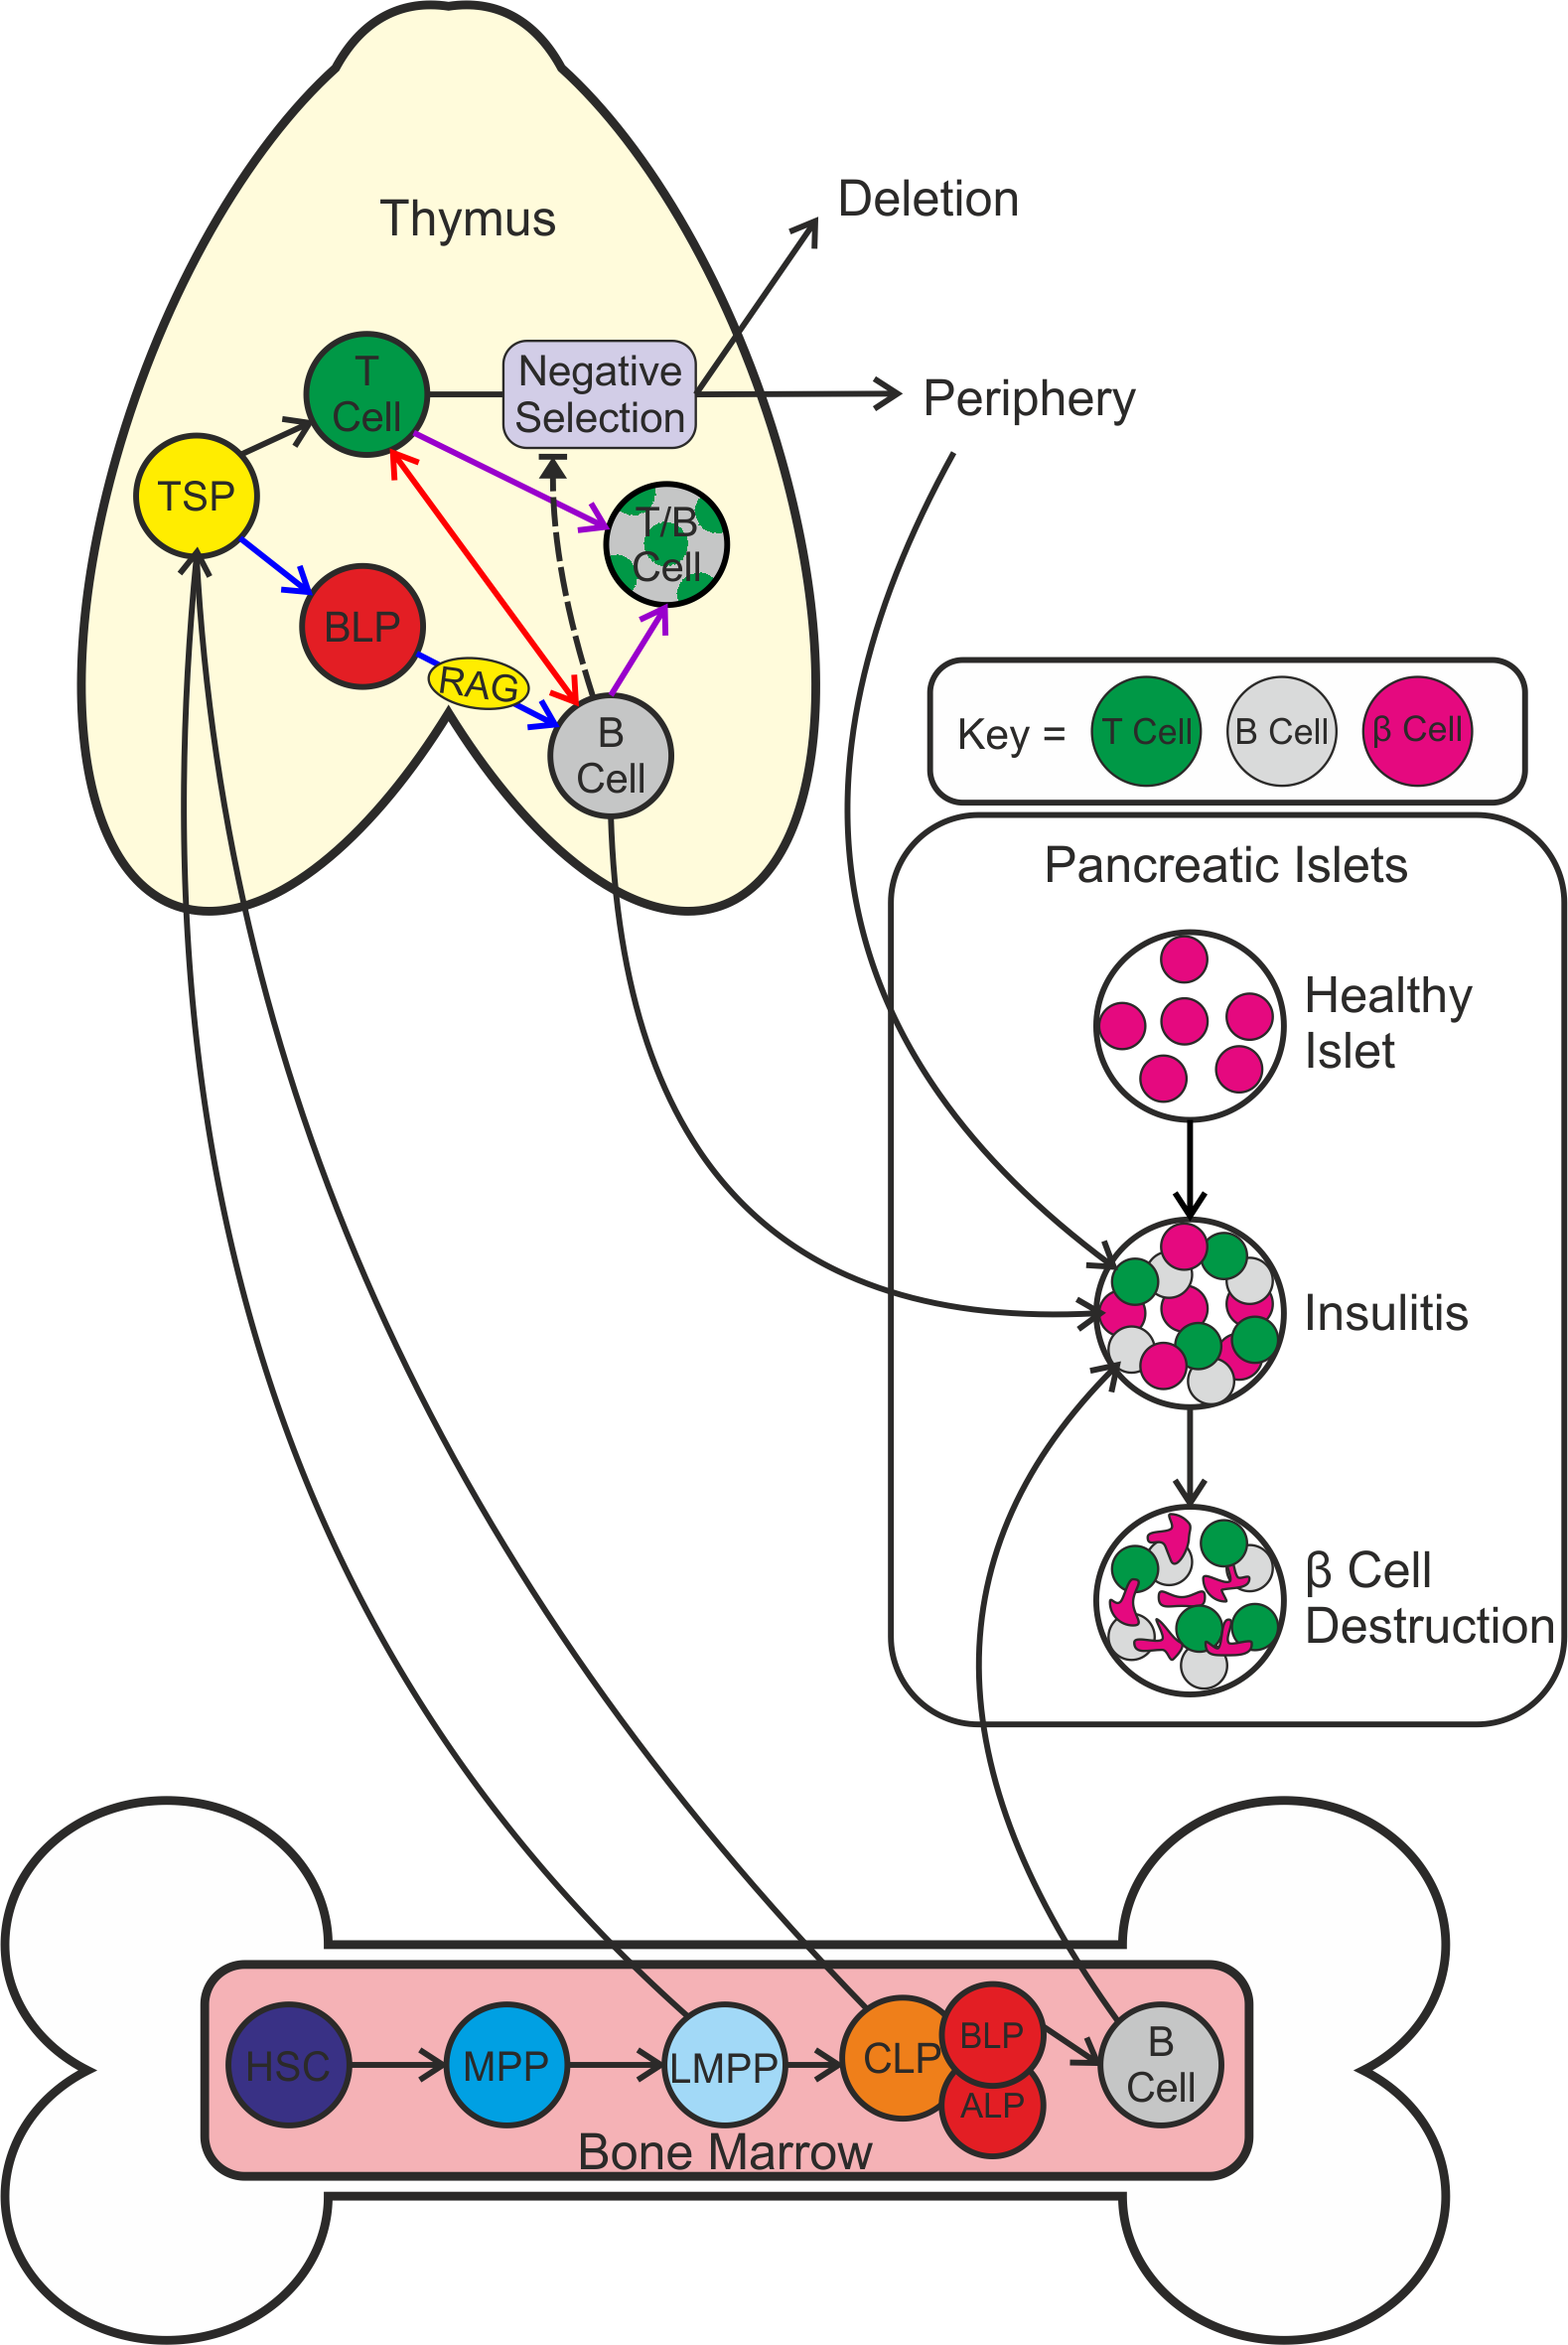
\includegraphics[width=\textwidth]{Figures/diagram2.png}
\caption{Diagrammatical summary. 
B cells develop in the bone marrow. 
T cells develop from thymic settling progenitors believed to be Flt3\textsuperscript{+}CCR7/9\textsuperscript{+} LMPPs or CLPs which migrate to the thymus.
Here they develop into T cells and pass through negative selection, for which the outcome is either clonal deletion or release into the periphery.
B cells may also be developing in the thymus, either following the same pathway as seen in the bone marrow (bone marrow), or from T cells developing into B cells (red arrows).
There also appears to be evidence of a cell expressing both T and B cell markers which may arise from a B or T cell that has been triggered to display both markers (purple arrows), or may be the mid point of a transitioning T or B cell.
Thymic B cells may contribute to insulitis.}
\label{fig:summarydiagram}
\end{figure}














